\chapter{Introduction}
\section{Motivation}
Many applications require a fast, structured data store. Correctly implementing
a custom solution in a general purpose programming language is a development cost.
Relational databases provide an attrative interface for describing the structure
and interfactions with a store, but come with performance caveats.
\\
\\ For example a common OLTP pattern is to use a database to store the current state of a service.
\begin{center}
    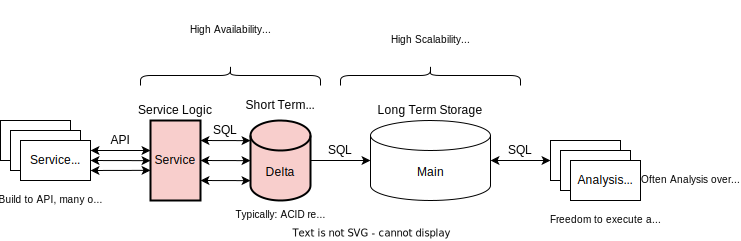
\includegraphics[scale=1.2]{_drawio/background/images/slow_delta.drawio.pdf}
\end{center}
\vspace{-1cm}
\noindent For many such applications the following holds.
\begin{enumerate}
    \setlength\itemsep{0em}
    \item Persistence requirements are weak enough to allow for in-memory only storage (optionally durability by replication).
    \item Each instance of the application is the sole interactor with the data store.
    \item Invariants/Constraints about the data must be maintained by the store.
    \item The schema and parameterized queries used are known at compile time. \label{lab:known_queries_item}
\end{enumerate}
A spectrum of solutions exist to embed a store in an application, here generally placed according to the strength of abstraction provided.
\begin{center}
    \includegraphics[width=\textwidth]{_drawio/introduction/images/problem_space.drawio.pdf}
\end{center}
Unfortunately the strongest abstractions are present in embedded databases that do not take advantage of \ref{lab:known_queries_item} as by design they both support shcema changes, and are independent from the host language (for example duckDB is embedable in Python, Java, Julia (and other) applications).
\\
\\
An ideal system would allow such a datastore to be expressed in a query language, with an embeddable
implementation generated for use, and optimised using the full knowledge of the query set \& schema.
\begin{center}
    \includegraphics[width=\textwidth]{_drawio/introduction/images/ideal_system.drawio.pdf}
\end{center}
\noindent
No such ideal system exists. The purpose of this project is to develop a
prototype for such a system and to demonstrate:
\begin{itemize}
    \setlength\itemsep{0em}
    \item Logical optimisation only possible from knowledge of the entire parameterised query set.
    \item Easy integration of such a store into existing applications.
    \item Expressed using the host language to allow its compiler to optimise the generated code, and fully integrate with the application (including inlining database code into application code).
\end{itemize}
We can show the potential upside of such optimisation by comparing the aforementioned sqlite and duckDB
in-memory embedded databases against both a naive and \textit{foresight} implementations.
\begin{center}
    \begin{tabular}{l p{.8\textwidth}}
        \textbf{naive}     & Implemented assuming the provided queries are only a subset of all required. As a result data structures supporting insert, update and deletion are required. \\
        \textbf{foresight} & Implemented assuming provided queries are the only queries required (as is the case for emdb).                                                                \\
    \end{tabular}
\end{center}
The schema used is as follows:
\begin{minted}{rust}
database! {
    // Reasoning:
    //  - Constraint checking required, needs to fail immediately (hybrid IVM)
    //  - premium is immutable, and iterated over. So we can maintain a view of
    //    two tables for premium & non-premium users
    //  - Very simple table
    table users {
        name: String,
        premium: bool,
        credits: i32,
    } @ [
        genpk(id),
        pred(premium || credits > 0) as prem_credits,
    ]
\end{minted}
Both sqlite and duckdb support \mintinline{SQL}{CHECK} constraints for \mintinline{rust}{prem_credits},
in sqlite an \mintinline{SQL}{AUTOINCREMENT} constraint is used for id. In DuckDB a default value
attached to a sequence is used to increment for every insert.
\\
\\ For the naive and foresight implementations we must ensure all writes are checked in advance to ensure the constraint is maintained, or the entire query has no effect.
When multiple rows are changed, this includes iterating through and pre-generating results before applying any.
\begin{minted}{rust}
    // Description:
    //   Create a row, pipe to insert, insert returns gen_pk id
    // Reasoning:
    //   - Needed for data insert, generation of id only occurs from here,
    //     hence we know the table alone determines id
    //   - Move semantics (taking ownership of data structure from outside the database)
    query new_user(username: String, prem: bool) {
        row(name: String = username, premium: bool = prem, credits: i32 = 0 )
            |> insert(users)
            ~> return;
    }
\end{minted}

\begin{minted}{rust}
    // Description
    //   Get an individual user's data.
    // Reasoning:
    //   - Performance reliant on access to users data structure
    //     hence need to make a good choice of mapping (user id -> data) here.
    query get_info(user_id: usize) {
        use users
            |> unique(use user_id as id)
            ~> return;
    }

    // Description:
    //    Get a snapshot of the entire users table state
    // Reasoning:
    //    - We can collect the database to a single structure decided by the compiler.
    //    - This can be radically sped up by removing copying of the string (no row deletions,
    //      immutable attribute, return reference bound to lifetime of database).
    //    - choosing a data structure for `users` table that is good for iteration
    query get_snapshot() {
        use users
            |> collect()
            ~> return;
    }

    // Description
    //   Update a given user's credits
    // Reasoning:
    //   - Need to apply constraint immediately
    //   - Need to index data structure
    //   - Database can see only credits is updated
    query add_credits(user: usize, creds: i32) {
        ref users
            |> unique(use user as id)
            ~> update(it use credits = credits + creds);
    }

    // Description:
    //   Apply multiplier bonus to premium users, and return the number of credits added
    // Reasoning:
    //   - Applying function over a tight loop
    //   - Iteration advantage form splitting premium users & non-premium
    //   - can be inlined to very simple iterate over &mut and increment sum
    query reward_premium(cred_bonus: f32) {
        ref users
            |> filter(it.premium)
            |> map(user: users::Ref = it, new_creds: i32 = ((it.credits as f32) * cred_bonus) as i32)
            |> update(it use credits = new_creds)
            |> map(creds: i32 = new_creds)
            |> fold((sum: i64 = 0) => (sum = sum + creds))
            ~> return;
    }

    // Description:
    //   Get the total number of credits in the premium table
    // Reasoning:
    //   Easy IVM case, all updates & inserts just need to add difference to
    //   the view
    query total_premium_credits() {
        use users
            |> filter(premium)
            |> map(credits: i64 = credits)
            |> fold((sum: i64 = 0) => (sum = sum + credits))
            ~> return;
    }
}    
\end{minted}
\section{Objectives}

\section{Contributions}
